\documentclass{beamer}
\usetheme{metropolis}           % Use metropolis theme
\usepackage{graphicx}
\usepackage{subcaption}
\title{Optimizing a Minimal Language using Pre-trained Language Models}
\date{}
\author{Ajay Narayanan}
\institute{Technical University of Munich}
\begin{document}
  \maketitle

\begin{frame}{Agenda}
	\tableofcontents
\end{frame}

\section{Introduction}

% Slide 1: Purpose of Language
\begin{frame}{The Purpose of Language}
	\begin{itemize}
		\item Human language evolved to aid survival and propagation.
		\item Facilitates collaboration, competition, and influence.
		\item Language is shaped by the trade-off between:
		\begin{itemize}
			\item \textbf{Expressiveness}
			\item \textbf{Efficiency} (driven by evolution)
		\end{itemize}
	\end{itemize}
\end{frame}

% Slide 2: Why Natural Languages Are Not Optimal
\begin{frame}{Why Natural Languages Are Not Optimal}
	\begin{itemize}
		\item Real-world communication happens in noisy environments.
		\item Redundancy helps with error correction.
		\item Natural languages are constrained by:
		\begin{itemize}
			\item Incremental language processing
			\item Need for compositionality, systematicity, and concatenation
		\end{itemize}
		\item Not optimal in the information-theoretic sense.
	\end{itemize}
\end{frame}

% Slide 3: Constructed Languages (ConLangs)
\begin{frame}{Constructed Languages (ConLangs)}
	\begin{itemize}
		\item Intentionally created languages.
		\item Types:
		\begin{itemize}
			\item Auxiliary (e.g. Esperanto)
			\item Fictional (e.g. Dothraki, Quenya, Klingon)
			\item Logical (e.g. Lojban)
			\item Minimalist (e.g. Toki Pona)
			\item Expressive (e.g. Ithkuil)
		\end{itemize}
	\end{itemize}
\end{frame}

% Slide 4: Defining Optimality
\begin{frame}{What Does "Optimal" Mean for a Language?}
	\begin{itemize}
		\item Information-theoretic efficiency
		\item Ease of learning
		\item Expressiveness
		\item Robustness in noisy conditions
		\item Ability to convey complex ideas
		\item \textbf{Key Questions:}
		\begin{itemize}
			\item Can we define and measure these?
			\item Can we build languages optimizing for one or more of these constraints?
		\end{itemize}
	\end{itemize}
\end{frame}

% Slide 5: Role of Large Language Models
\begin{frame}{Can LLMs Help Design Better Languages?}
	\begin{itemize}
		\item LLMs encode deep patterns in natural language and world knowledge.
		\item They may uncover latent linguistic structures.
		\item Potential use in evaluating or designing:
		\begin{itemize}
			\item Phonology, orthography, morphology
			\item Syntax and vocabulary
		\end{itemize}
		\item Could LLMs help define and optimize linguistic trade-offs?
		\item Could LLMs assist in the language generation process?
	\end{itemize}
\end{frame}

% Slide 6: Thesis Goals
\begin{frame}{Thesis Goals}
	\begin{enumerate}
		\item Define linguistic optimality across dimensions.
		\item Explore design of an efficient constructed language.
		\item Investigate how LLMs can aid this process.
	\end{enumerate}
\end{frame}

\section{Methodology}

% Slide 1: Methodological Overview
\begin{frame}{Methodological Overview}
	\begin{itemize}
		\item Step-by-step approach inspired by language construction literature.
		\item Language specification includes:
		\begin{itemize}
			\item Phonemic inventory
			\item Phonotactics
			\item Grammar
			\item Vocabulary
		\end{itemize}
		\item Translation of known texts used for evaluation.
	\end{itemize}
\end{frame}

% Slide 2: Research Design
\begin{frame}{Research Design}
	\begin{itemize}
		\item Modular, computational experimental design.
		\item Objective: Guide LLMs to generate human-like ConLangs.
		\item Pipeline consists of:
		\begin{itemize}
			\item Phonology
			\item Morphology
			\item Syntax
			\item Vocabulary
		\end{itemize}
		\item Allows ablative analysis and future extensibility.
	\end{itemize}
\end{frame}

% Slide 3: Modular Language Generation Pipeline
\begin{frame}{Language Generation Pipeline}
	\begin{itemize}
		\item Modules operate sequentially or in parallel with shared dependencies.
		\item Each module is an independent variable.
		\item Enables targeted experimentation to study:
		\begin{enumerate}
			\item Effect of phoneme inventory size
			\item Influence of phonotactic rules
			\item Impact of grammatical structure
			\item Variation in vocabulary generation
		\end{enumerate}
	\end{itemize}
\end{frame}

% Slide 4: Evaluation Framework
\begin{frame}{Evaluation Framework}
	\begin{itemize}
		\item Evaluation modules benchmark generated languages.
		\item Results stored alongside each language.
		\item Three main categories:
		\begin{itemize}
			\item Information Loss
			\item Simplicity
			\item Zipf's Law Compliance
		\end{itemize}
	\end{itemize}
\end{frame}

% Slide 5: Information Loss Metrics
\begin{frame}{Information Loss Metrics}
	\begin{itemize}
		\item \textbf{Machine Translation Scores}:
		\begin{itemize}
			\item Round-trip translation using LLM
			\item Evaluated with BLEU, ROUGE, METEOR
		\end{itemize}
		\item \textbf{Reading Comprehension}:
		\begin{itemize}
			\item LLM answers questions based on original and translated texts
			\item Score = \% of correct answers
		\end{itemize}
	\end{itemize}
\end{frame}

% Slide 6: Simplicity Metrics
\begin{frame}{Simplicity Metrics}
	\begin{itemize}
		\item \textbf{BERT Fine-tuning}: Measures perplexity of model trained on new language.
		\item \textbf{Vocabulary Size}: Total lexicon count.
		\item \textbf{Phonemic Inventory Size}: Number of phonemes used.
		\item \textbf{Phonotactic Complexity}: Assesses rule complexity.
	\end{itemize}
\end{frame}

% Slide 7: Zipf's Law Metric
\begin{frame}{Zipf's Law Metric}
	\begin{itemize}
		\item Evaluates how closely the generated language follows Zipf’s Law.
		\item Zipf exponent compared against that of the original English text.
		\item Indicator of natural distribution of word frequencies.
	\end{itemize}
\end{frame}

\section{System Design and Implementation}

% Slide 1
\begin{frame}{Pipeline Overview}
	\begin{itemize}
		\item Modular architecture for conlang generation.
		\item Core object: \texttt{LanguageDescription}.
		\item Pipeline managed by subclassing \texttt{Pipeline}.
		\item JSON-based output for module results.
	\end{itemize}
\end{frame}

% Slide 2
\begin{frame}{Module Design}
	\begin{itemize}
		\item Each module subclasses \texttt{Module}.
		\item Implements \texttt{execute()} method.
		\item Can add/modify language features.
		\item Checks dependencies and raises errors if needed.
	\end{itemize}
\end{frame}

% Slide 3
\begin{frame}{Phonetics and Phonotactics}
	\textbf{Phonetics Module}
	\begin{itemize}
		\item Based on PHOIBLE phoneme segments.
		\item \texttt{MostCommonPhonemesModule}.
	\end{itemize}
	\textbf{Phonotactics Module}
	\begin{itemize}
		\item \texttt{BasicPhonotacticsModule} for C/V structures.
		\item \texttt{CustomPhonotacticsModule} supports constraints.
	\end{itemize}
\end{frame}

% Slide 4
\begin{frame}{Grammar Modules}
	\begin{itemize}
		\item Features via \texttt{GrammaticalFeatures} class.
		\item Uses \texttt{AbstractFeature} and \texttt{AbstractPOS}.
		\item Modules:
		\begin{itemize}
			\item \texttt{BaselineAgglutinativeGrammarModule}
			\item \texttt{BaselineIsolatingGrammarModule}
		\end{itemize}
	\end{itemize}
\end{frame}

% Slide 5
\begin{frame}{Vocabulary Modules}
	\begin{itemize}
		\item Data in \texttt{VocabDictionary}.
		\item Generation:
		\begin{itemize}
			\item \texttt{FromSourceVocabularyModule}
			\item \texttt{ClusterTwoLevelVocabularyModule}
			\item \texttt{ClusterAndSimplifyVocabularyModule}
			\item \texttt{ApproximatingVocabularyModule}
		\end{itemize}
		\item Mapping:
		\begin{itemize}
			\item \texttt{RandomMappingModule}
		\end{itemize}
	\end{itemize}
\end{frame}

% Slide 6
\begin{frame}{Translation Module}
	\begin{itemize}
		\item Translates using LLMs.
		\item Paragraph-level translation of \texttt{AbstractSourceText}.
	\end{itemize}
\end{frame}

% Slide 7
\begin{frame}{Evaluation Framework}
	\begin{itemize}
		\item Evaluations handled by \texttt{Evaluator} class.
		\item Independent of the main pipeline.
		\item Outputs saved in an \texttt{evaluations} folder.
	\end{itemize}
\end{frame}

% Slide 8
\begin{frame}{Evaluation Modules}
	\begin{itemize}
		\item \textbf{Translation Quality:}
		\begin{itemize}
			\item \texttt{DetranslationEvaluator} (BLEU, METEOR, ROUGE)
			\item \texttt{GenerateTranslationSummary}
		\end{itemize}
		\item \textbf{Compression and Comprehension:}
		\begin{itemize}
			\item \texttt{CompressionEvaluator}
			\item \texttt{RaceCEvaluator}
		\end{itemize}
		\item \textbf{Learnability and Naturalness:}
		\begin{itemize}
			\item \texttt{BertEvaluator}
			\item \texttt{ZipfsLawEvaluator}
		\end{itemize}
	\end{itemize}
\end{frame}

% Slide 9
\begin{frame}{Pipeline Variants}
	\begin{itemize}
		\item \textbf{Baseline:} Most common phonemes, CV rules.
		\item \textbf{Approximation:} Fixed vocabulary + embedding-based matching.
		\item \textbf{Two-Level:} Bi-syllabic clustering-based vocabulary.
		\item \textbf{Cluster \& Simplify:} One word per cluster.
		\item \textbf{Phonotactics:} Custom syllable constraints.
	\end{itemize}
\end{frame}

% Slide 10
\begin{frame}{LLMs and Embedding Models}
	\begin{itemize}
		\item \textbf{Local LLMs:} via Ollama, e.g. \texttt{deepseek-r1:14b}.
		\item \textbf{Remote LLMs:} OpenAI and Groq (\texttt{gpt-4o}).
		\item \textbf{Embeddings:} \texttt{all-MiniLM-L6-v2}.
	\end{itemize}
\end{frame}

% Slide 11
\begin{frame}{Clustering Methods}
	\begin{itemize}
		\item Subclasses of \texttt{ClusteringMethod}.
		\item Vocabulary clustering: \texttt{AgglomerativeClustering}.
		\item Alternatives supported: KMeans, DBScan, HDBScan.
	\end{itemize}
\end{frame}

% Slide 12
\begin{frame}{Datasets and Tools}
	\begin{itemize}
		\item Dataset: \texttt{RaceC} (Race-C dataset).
		\item Word frequency: \texttt{wordfreq} library.
		\item Corpus source: Exquisite Corpus.
		\item Outputs: HTML summaries and translation pairs.
	\end{itemize}
\end{frame}

\section{Results and Evaluation}

% Slide: Introduction
\begin{frame}{Overview}
	\begin{itemize}
		\item Discusses key experimental results.
		\item Evaluates effects of parameters on performance.
		\item Summarizes findings.
		\item Outlines directions for future work.
	\end{itemize}
\end{frame}

% Slide: Effect of Phoneme Count
\begin{frame}{Effect of Phoneme Count}
	\begin{itemize}
		\item Minimal impact on translation or Race-C scores.
		\item Suggests that languages can be simplified in phoneme inventory.
		\item Meaning preservation not significantly affected.
	\end{itemize}
	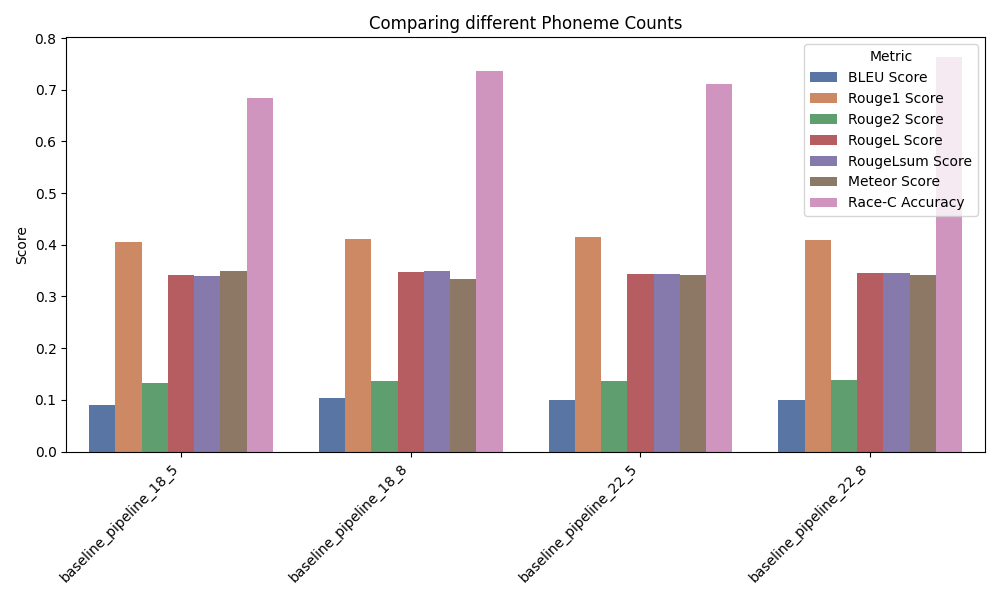
\includegraphics[width=0.7\linewidth]{figures/results/1_effect_of_phoneme_count.png}
\end{frame}

% Slide: Effect of Phonotactics
\begin{frame}{Effect of Phonotactics}
	\begin{itemize}
		\item Simplified phonotactic rules do not degrade performance.
		\item Translation and comprehension scores largely unaffected.
		\item Simplification viable for phonological structure.
	\end{itemize}
	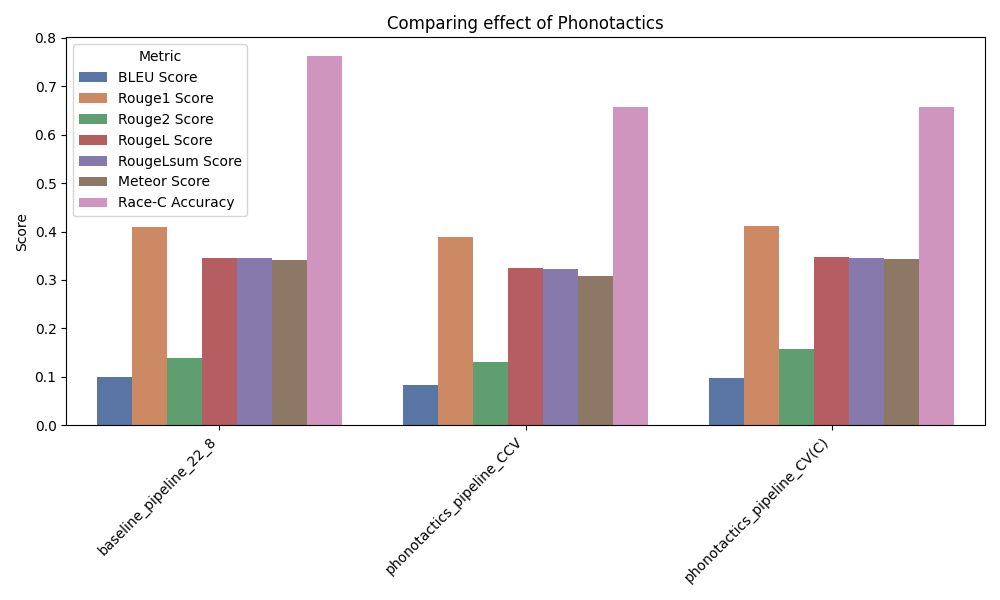
\includegraphics[width=0.7\linewidth]{figures/results/1_effect_of_phonotactics.png}
\end{frame}

% Slide: Effect of Grammar Rules
\begin{frame}{Effect of Grammar Rules}
	\begin{itemize}
		\item Compared Agglutinative vs. Isolating grammars.
		\item No major difference in translation or comprehension.
		\item Only Bert perplexity varied—needs further analysis.
	\end{itemize}
	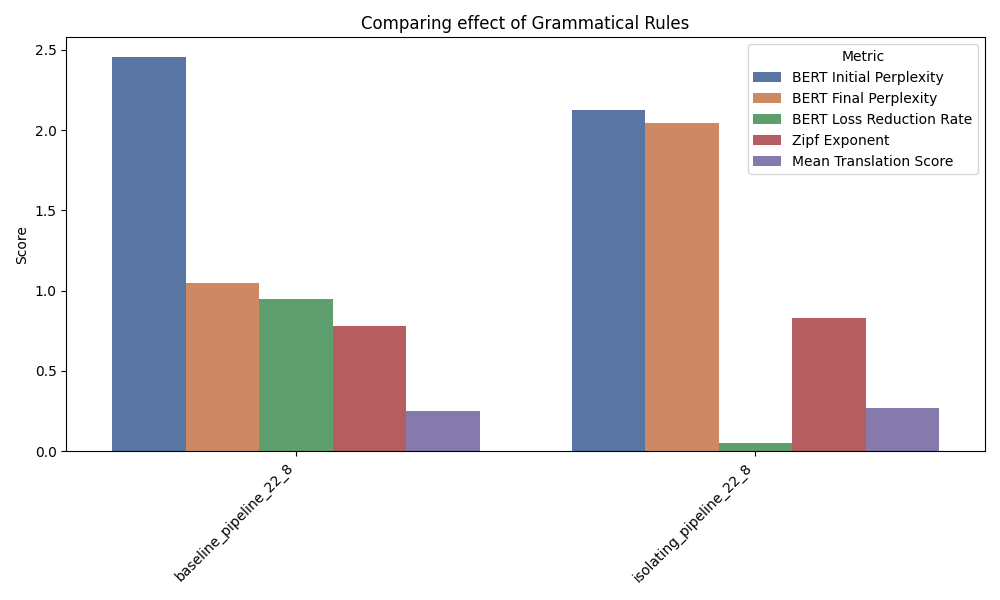
\includegraphics[width=0.7\linewidth]{figures/results/1_effect_of_grammar.png}
\end{frame}

% Slide: Effect of Vocabulary Generation Methods (1/2)
\begin{frame}{Vocabulary Simplification and Performance}
	\begin{itemize}
		\item Vocabulary simplification causes performance drop.
		\item MTS (n-gram) suffers more than Race-C (meaning-based).
		\item Ratio of score to vocab size is better for simpler vocab methods.
	\end{itemize}
\end{frame}

% Slide: Effect of Vocabulary Generation Methods (2/2)
\begin{frame}{Effect of Simplified Vocabulary}
	\begin{columns}
		\column{0.48\textwidth}
		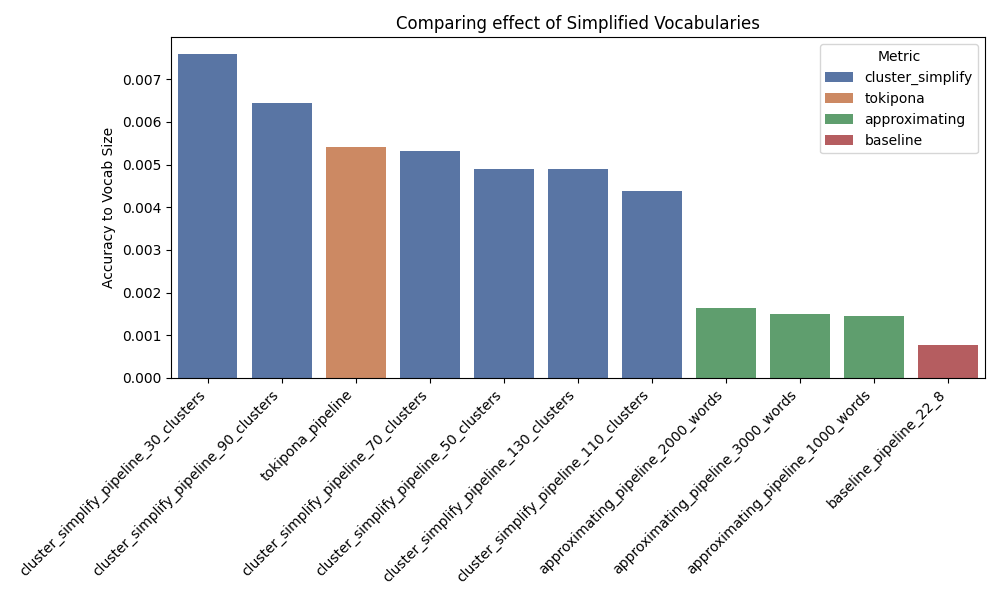
\includegraphics[width=\linewidth]{figures/results/1_effect_of_vocab_simplify.png}
		\captionof{figure}{Race-C Accuracy}
		\column{0.48\textwidth}
		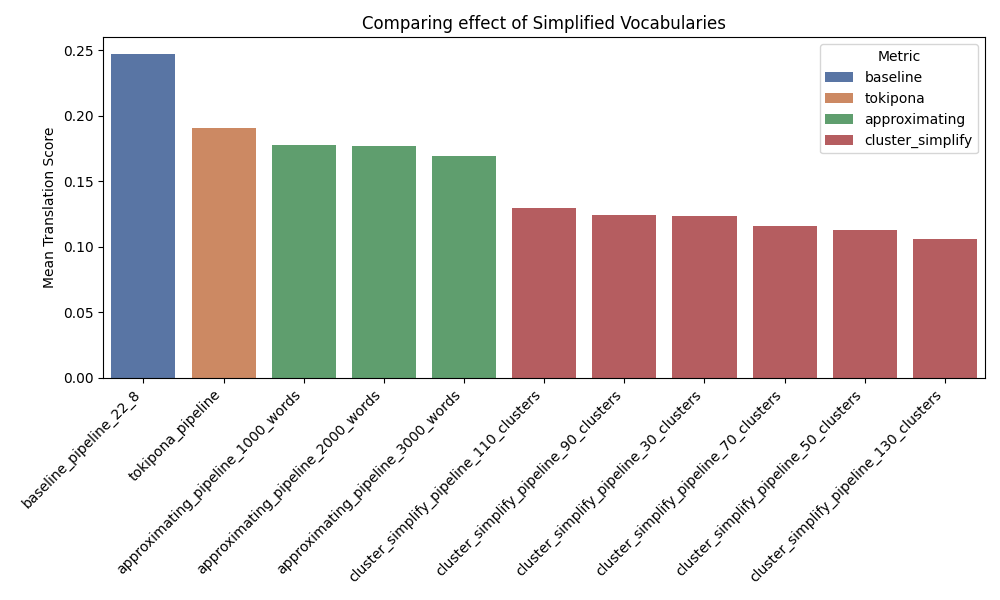
\includegraphics[width=\linewidth]{figures/results/1_effect_of_vocab_simplify_mts.png}
		\captionof{figure}{Mean Translation Score (MTS)}
	\end{columns}
\end{frame}

% Slide: Effect of Model Temperature
\begin{frame}{Effect of Language Model Temperature}
	\begin{itemize}
		\item High temperature leads to less consistent results.
		\item Low to moderate values (e.g., 0.2) are stable.
		\item Reproducibility improves with lower temperature.
	\end{itemize}
	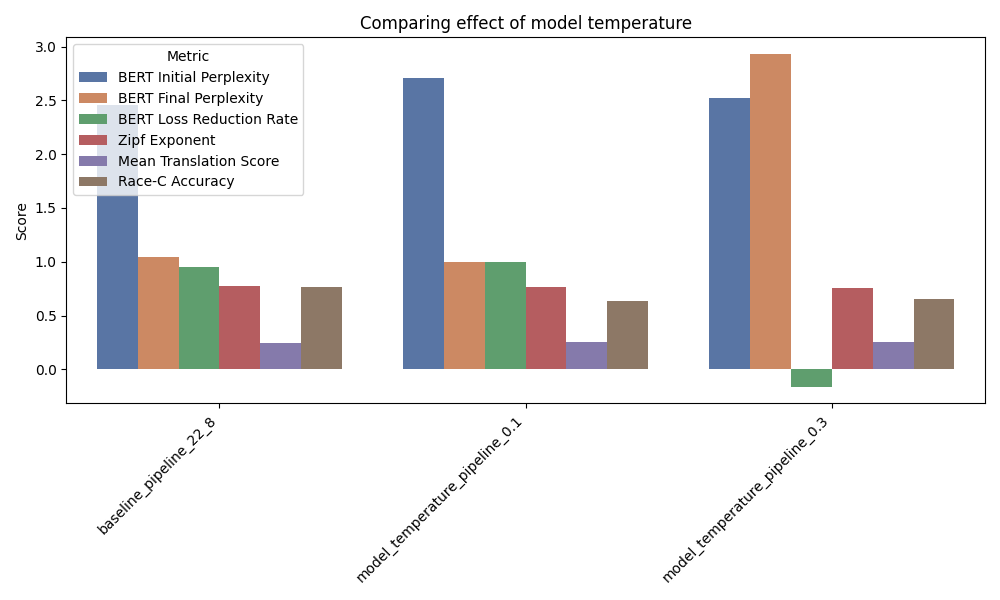
\includegraphics[width=0.7\linewidth]{figures/results/1_effect_of_model_temperature.png}
\end{frame}

\section{Conclusion}

% Slide: Conclusion
\begin{frame}{Conclusion}
	\begin{itemize}
		\item LLMs can aid in building efficient, minimal conlangs.
		\item Simplification is possible in phonology, grammar, and vocab.
		\item Reading comprehension is robust even with simplification.
		\item Zipf-like distributions emerged naturally.
		\item Framework enables modular experimentation and evaluation.
	\end{itemize}
\end{frame}

% Slide: Future Work
\begin{frame}{Future Work}
	\begin{itemize}
		\item Explore more grammar/vocab generation strategies.
		\item Better metrics for simplicity and efficiency.
		\item Deeper analysis of grammatical influence on meaning retention.
		\item Extend to spoken or multi-modal languages.
	\end{itemize}
\end{frame}

\begin{frame}{Questions?}
	\centering
	Thank you!\\
	Questions are welcome.
\end{frame}

\end{document}